\documentclass[12pt, letterpaper]{article}

\usepackage{graphicx}
\usepackage{caption}
\usepackage{amsmath}
\usepackage{amsfonts}
\captionsetup[figure]{font=small, labelfont=bf}

\title{Compton Scattering}
\author{Jay Shen}
\date{December 2024}

\begin{document}

\maketitle

\section{Results}

In this lab we evaluate the quantum mechanical model for scattering proposed by Compton. The sensitivity of the model necessitates calibrating our measurements to be as accurate as possible. Thus, our effort here is two-fold: precise calibration of spectrum measurements and an empirical evaluation of the Compton model. 

\subsection{Calibration}

To calibrate our measurements, we first collect gamma spectra from a variety of radioactive sources. Then, we measure the location of the full peaks in the channel units of the PHA software. The expectation is that Channel is predictive of Energy, so we then compare our channel measurements to the expected energies of the peaks, and try to derive some relation between them. 

We measure full peak location by visually determining an interval within which the peak falls and fitting a Gaussian function to the spectrum data: 
\[
    y = \frac{A}{\sigma \sqrt{2 \pi}} \: \exp[- \frac{(x - \mu)^2}{2 \sigma^2}] + mx + b
\]
We can then extract the fitted mean which represents the peak location. The PHA software provides uncertainties on the spectrum data, and our regression software is able to propagate this to its fitted parameters. 

\begin{figure}[!h]
    \centering
    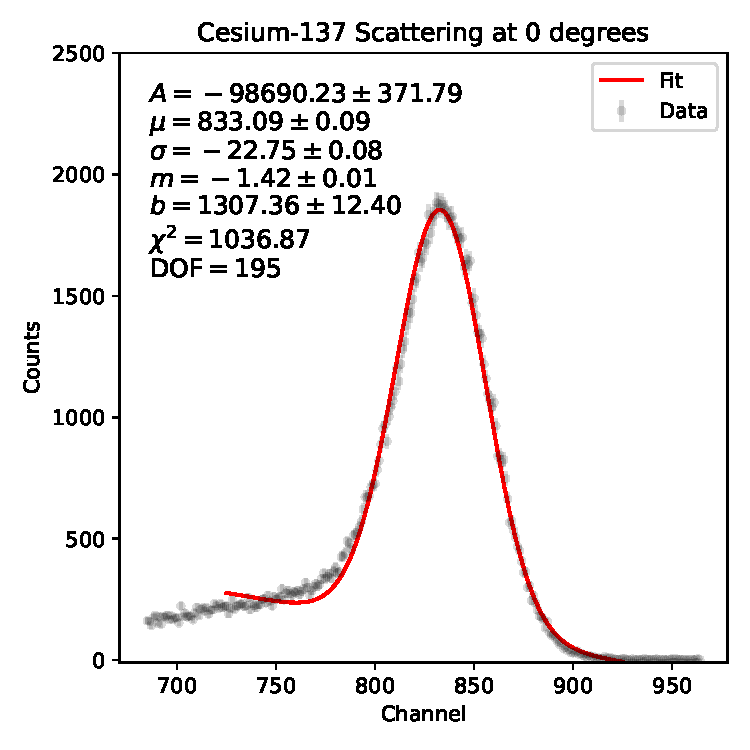
\includegraphics[width=0.75\textwidth]{experiment2/figures/scattering3/0.pdf}
    \caption{Scattering of Cesium-137 gammas at 0 degrees. A Gaussian + Linear function is fit to the data. Function parameters are listed. }
    \label{fig:scattering-0}
\end{figure}

Figure \ref{fig:scattering-0} shows an example of fitting such a function to a Cesium-137 full energy peak. The location of the peak in channels is given by $\mu$. 

We repeat this fitting step on a range of radioactive sources which exhibit peaks of various energies. Table \ref{table:calibration3} lists some of this collected data. 

\begin{table}[!h]
\footnotesize
\centering
\begin{tabular}{| c c | c c | c |}
    \hline
    Source & Energy & Centroid & Gain & \textbf{Channel} \\
    \hline
    Cs-137 & $662.00 \pm 1.00$ & $877.98 \pm 0.06$ & 2 & $438.99 \pm 0.03$\\
    Cs-137 & $32.00 \pm 1.00$ & $44.29 \pm 0.03$ & 2 & $22.14 \pm 0.01$\\
    Na-22 & $511.00 \pm 1.00$ & $682.08 \pm 0.11$ & 2 & $341.04 \pm 0.06$ \\
    Am-241 & $59.54 \pm 1.00$ & $81.67 \pm 0.01$ & 2 & $40.84 \pm 0.01$ \\
    Ba-133 & $31.00 \pm 1.00$ & $40.34 \pm 0.02$ & 2 & $20.17 \pm 0.01$ \\
    Ba-133 & $81.00 \pm 1.00$ & $110.85 \pm 0.05$ & 2 & $55.42 \pm 0.03$ \\
    Ba-133 & $356.00 \pm 1.00$ & $468.44 \pm 0.16$ & 2 & $234.22 \pm 0.08$ \\
    Co-57 & $122.00 \pm 1.00$ & $163.72 \pm 0.22$ & 2 & $81.86 \pm 0.11$ \\
    \hline
\end{tabular}
\caption{
    Table of calibration measurements. ``Energy" denotes the theoretical expectation peak energy. ``Centroid" again denotes the fitted peak mean $\mu$ and $\text{Channel}=\text{Centroid}/\text{Gain}$. 
}
\label{table:calibration3}
\end{table}

Then, we can fit a curve to this data to obtain a map between channel and energy. It turns out that a simple linear function suffices. As shown in \ref{fig:calibration3}, the linear model fits this data very well, and achieves a reduced $\chi^2$ score of $4.42$, which is reasonably close to $1$, indicating good fit. 

\begin{figure}[!h]
    \centering
    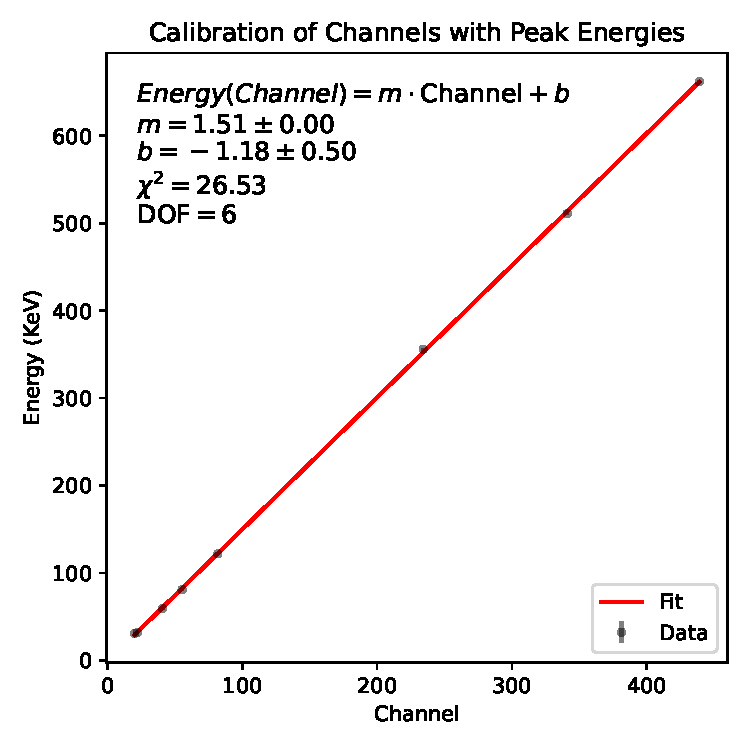
\includegraphics[width=0.75\textwidth]{experiment2/figures/calibration_3.pdf}
    \caption{Measured pulse channel versus theoretical expectation energy.}
    \label{fig:calibration3}
\end{figure}

We now have a function
\[\text{Energy}=m \cdot \text{Channel} +b\]
mapping channels to energy allowing us to calibrate our data. The uncertainties in these calibrations can be computed using:
\[(\delta \text{Energy})^2 = \text{Channel}^2 \cdot (\delta m)^2 + m^2 \cdot (\delta \text{Channel})^2 + (\delta b)^2\]
The uncertainties $\delta m$ and $\delta b$ are computed by the regression software, which propagates the uncertainties in the channel and energy measurements. The uncertainty $\delta \text{Channel}$ is also given by the regression software when it fit the Gaussian curve to the spectrum data. 

\subsection{Scattering Data}

To evaluate the accuracy of the Compton model and our own setup, we will scatter radiation from a Cesium-137 source and collect spectra from various angles. One such spectrum is shown in Figure \ref{}. Then we determine the full peak location, calibrate those measurements to obtain a set of energies, and analyze their relation to the scattering angles. 

\begin{figure}[!h]
    \centering
    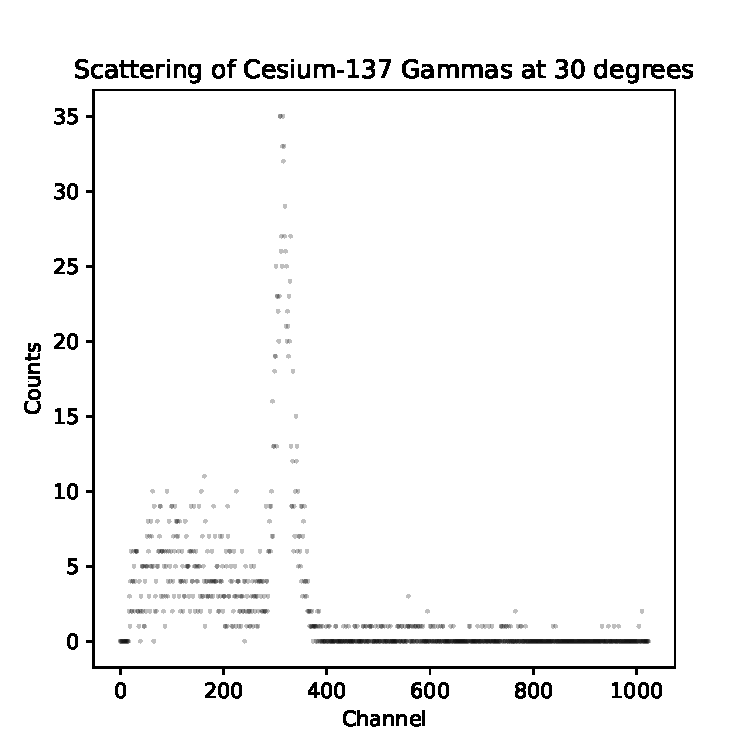
\includegraphics[width=0.75\textwidth]{experiment2/figures/scattering1-30.pdf}
    \caption{Calibration functions fit on data from Time 0 and Time 1.}
    \label{fig:gain-drift}
\end{figure}

A preliminary set of data is listed in Table \ref{table:scattering1}. Here, in the interest of time, we did not fit Gaussian curves to obtain the location of the full peaks, rather we rely on the PHA software's centroid functionality. This tends to give accurate measurements with wider margins of error, which are fine for our use now. We compute the energy using the calibration method described above and obtain uncertainty estimates. 

\begin{table}[!h]
\footnotesize
\centering
\begin{tabular}{| c | c c | c c |}
    \hline
    $\theta$ (deg) & Centroid & Gain & Channel & Energy \\
    \hline
    0 & $419 \pm 1$ & 1 & $419.00 \pm 1.00$ & $777.50 \pm 2.01$ \\
    30 & $318 \pm 1$ & 1 & $318.00 \pm 1.00$ & $585.39 \pm 1.98$ \\
    45 & $266 \pm 1$ & 1 & $266.00 \pm 1.00$ & $486.49 \pm 1.97$ \\
    60 & $223 \pm 1$ & 1 & $223.00 \pm 1.00$ & $404.70 \pm 1.96$ \\
    75 & $188 \pm 1$ & 1 & $188.00 \pm 1.00$ & $338.13 \pm 1.96$ \\
    90 & $162 \pm 1$ & 1 & $162.00 \pm 1.00$ & $288.68 \pm 1.96$ \\
    120 & $124 \pm 1$ & 1 & $124.00 \pm 1.00$ & $216.41 \pm 1.95$ \\
    \hline
\end{tabular}
\caption{Table of scattering measurements taken from setup with collimator. Centroid denotes the fitted peak mean $\mu$ and $\text{Channel}=\text{Centroid}/\text{Gain}$}
\label{table:scattering1}
\end{table}

In Figure \ref{fig:scattering-1}, these energies are plotted against the scattering angle from which they were taken. The expected Compton relation is shown as well. 

\begin{figure}[!h]
    \centering
    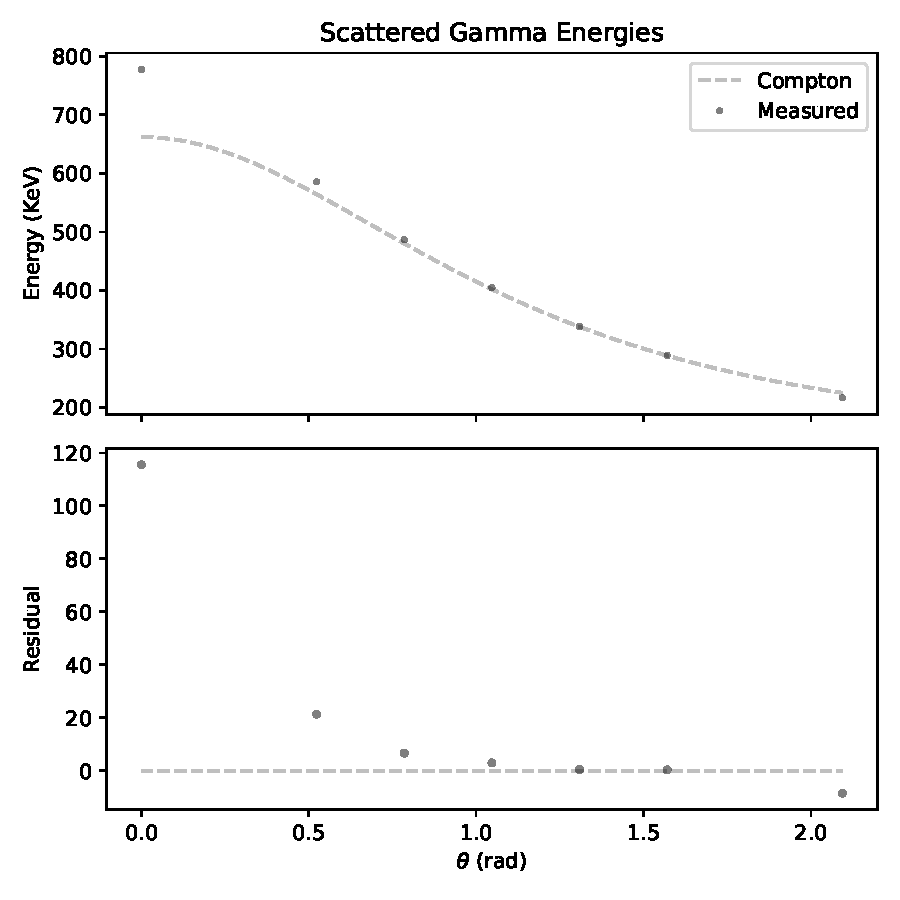
\includegraphics[width=0.75\textwidth]{experiment2/figures/scattering1.pdf}
    \caption{Evidently, the residual plot exhibits an exponential-decay-like trend. }
    \label{fig:scattering-1}
\end{figure}

From Figure \ref{fig:scattering-1}, we observe a systematic bias. There is a noticeable trend of large positive error near $\theta = 2 \pi n$ for $n \in \mathbb{Z}$, and low error near $\theta = \pi m$ for $m \in \mathbb{Z}$. We will evaluate this further in the next sections. 

\subsection{Systematic Bias: Calibration}

What is causing this systematic bias of our data from the expected Compton relation?

Our initial guess was that the issue lied in our calibration. It was unlikely our calibration functions failed to extrapolate, as we had explicitly included datapoints in the $662$ KeV energy scale in our calibration datasets. We hypothesized there was a bias introduced by the staggering of our measurements. We decided to test this by checking if calibrating at different times of the day produced different result. 

We took two calibrations an hour apart, emulating the time scale at which the scattering measurements were taken. Table \ref{table:gain-drift} shows the data collected at the two times. Figure \ref{fig:gain-drift} juxtaposes the two fitted calibration functions. 

\begin{table}[!h]
\footnotesize
\centering
\begin{tabular}{| c c | c c | c | c c | c |}
    \cline{3-8}
    \multicolumn{2}{c|}{} & \multicolumn{3}{c|}{Time 0} & \multicolumn{3}{c|}{Time 1} \\
    \hline
    Source & Energy & Centroid & Gain & \textbf{Channel} & Centroid & Gain & \textbf{Channel} \\
    \hline
    Cs-137 & $662.00 \pm 1.00$ & $873 \pm 1$ & 2 & $436.50 \pm 0.50$ & $895 \pm 1$ & 2 & $447.50 \pm 0.50$ \\
    Cs-137 & $32.00 \pm 1.00$ & $44 \pm 1$ & 2 & $22.00 \pm 0.50$ & $45 \pm 1$ & 2 & $22.50 \pm 0.50$ \\
    Na-22 & $511.00 \pm 1.00$ & $357 \pm 1$ & 1 & $357.00 \pm 1.00$ & $363 \pm 1$ & 1 & $363.00 \pm 1.00$ \\
    Na-22 & $1275.00 \pm 1.00$ & $830 \pm 1$ & 1 & $830.00 \pm 1.00$ & $851 \pm 1$ & 1 & $851.00 \pm 1.00$ \\
    Ba-133 & $31.00 \pm 1.00$ & $41 \pm 1$ & 2 & $20.50 \pm 0.50$ & $42 \pm 1$ & 2 & $21.00 \pm 0.50$ \\
    Ba-133 & $81.00 \pm 1.00$ & $114 \pm 1$ & 2 & $57.00 \pm 0.50$ & $117 \pm 1$ & 2 & $58.50 \pm 0.50$ \\
    Ba-133 & $356.00 \pm 1.00$ & $476 \pm 1$ & 2 & $238.00 \pm 0.50$ & $485 \pm 1$ & 2 & $242.50 \pm 0.50$ \\
    \hline
\end{tabular}
\caption{Calibration data taken at Time 0 and at Time 1, an hour later. }
\label{table:gain-drift}
\end{table}

\begin{figure}[!h]
    \centering
    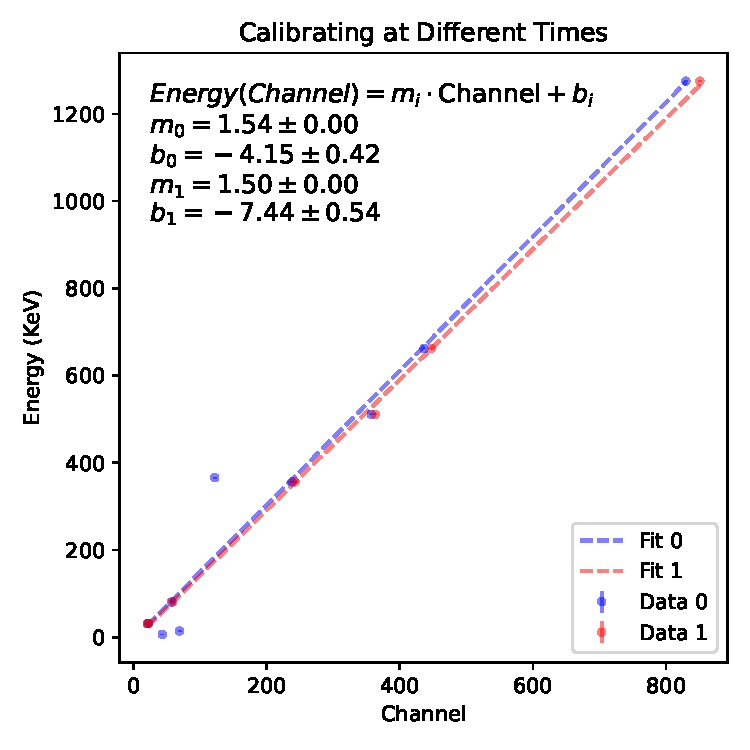
\includegraphics[width=0.75\textwidth]{experiment2/figures/gain-drift.pdf}
    \caption{Calibration functions fit on data from Time 0 and Time 1.}
    \label{fig:gain-drift}
\end{figure}

From visual inspection, we conclude that it is unlikely calibration drift plays a significant role in producing the bias. The differences between the two calibration curves are not significant enough to product the dramatic bias exhibited. 

\subsection{Systematic Bias: PMT Saturation}

After our initial guess was disqualified, we were given a hint to explore PMT saturation. PMT saturation occurs when the incoming gamma beam is too intense. The rate of photons entering the PMT begins to exceed the read frequency of the PMT and the pulses interfere, causing significant issues with the measurement. To solve this problem, we will block some of the incoming photons using a lead collimator. 

We take a set of scattering measurements, using the lead collimator for low angles where the beam is very intense. This data is listed in Table \ref{table:pmt-saturation} alongside our dataset from the collimator-less setup. 

\begin{table}[!h]
\footnotesize
\centering
\begin{tabular}{| c | c c | c c |}
    \cline{2-5}
    \multicolumn{1}{c|}{} & \multicolumn{2}{c|}{w/o Collimator} & \multicolumn{2}{c|}{w/ Collimator} \\
    \hline
    $\theta$ (deg) & Channel & Energy & Channel & Energy \\
    \hline
    0 & $419.00 \pm 1.00$ & $777.50 \pm 2.01$ & $416.55 \pm 0.05$ & $627.66 \pm 1.09$ \\
    15 & - & - & $411.99 \pm 0.11$ & $620.79 \pm 1.09$ \\
    30 & $318.00 \pm 1.00$ & $585.39 \pm 1.98$ & $354.83 \pm 0.15$ & $534.50 \pm 0.99$ \\
    45 & $266.00 \pm 1.00$ & $486.49 \pm 1.97$ & $304.89 \pm 0.14$ & $459.11 \pm 0.90$ \\
    60 & $223.00 \pm 1.00$ & $404.70 \pm 1.96$ & $258.70 \pm 0.14$ & $389.38 \pm 0.81$ \\
    75 & $188.00 \pm 1.00$ & $338.13 \pm 1.96$ & - & - \\
    90 & $162.00 \pm 1.00$ & $288.68 \pm 1.96$ & $189.83 \pm 0.15$ & $285.40 \pm 0.71$ \\
    105 & - & - & $169.66 \pm 0.24$ & $254.94 \pm 0.73$ \\
    120 & $124.00 \pm 1.00$ & $216.41 \pm 1.95$ & $151.98 \pm 0.23$ & $228.26 \pm 0.70$ \\
    \hline
\end{tabular}
\caption{Scattering data from setup without versus with lead collimator. Note that the two datasets were taken on different days. The calibration functions used are $\text{Energy} = 1.90 \cdot \text{Channel}-19.44$ and $\text{Energy} = 1.50 \cdot \text{Channel}-1.18$ for the setups without and with the collimator, respectively.}
\label{table:pmt-saturation}
\end{table}

We then juxtapose the two datasets. Evidently, the data taken from the setup with the collimator no longer exhibits the drastic bias we saw before. There still exists some sort of systematic bias, and interestingly it is now negative, though it is still generally worse around small angles. 

\begin{figure}[!h]
    \centering
    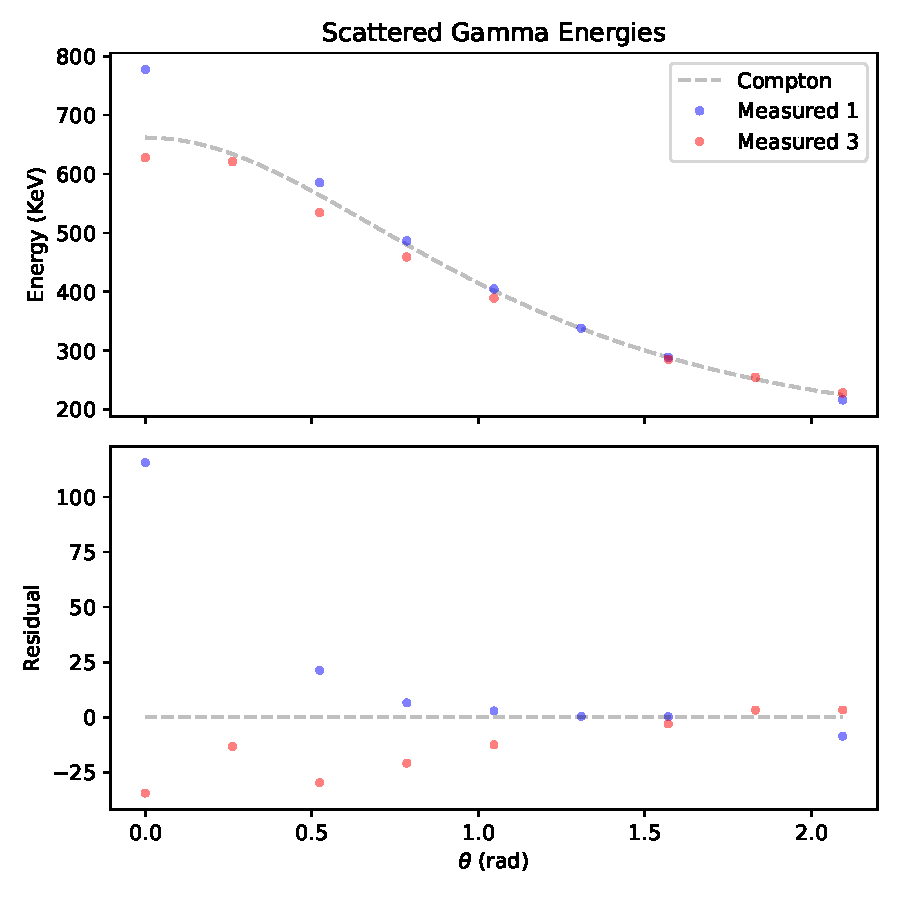
\includegraphics[width=0.75\textwidth]{experiment2/figures/pmt_saturation.pdf}
    \caption{Scattering data with collimator versus without. }
    \label{fig:pmt-saturation}
\end{figure}

\section{Conclusions}

To conclude our inquiry, we fit the Compton curve to our data, letting the rest mass vary. Figure \ref{fig:compton-fit} shows this resulting curve next to the expected Compton curve. 

\begin{figure}[!h]
    \centering
    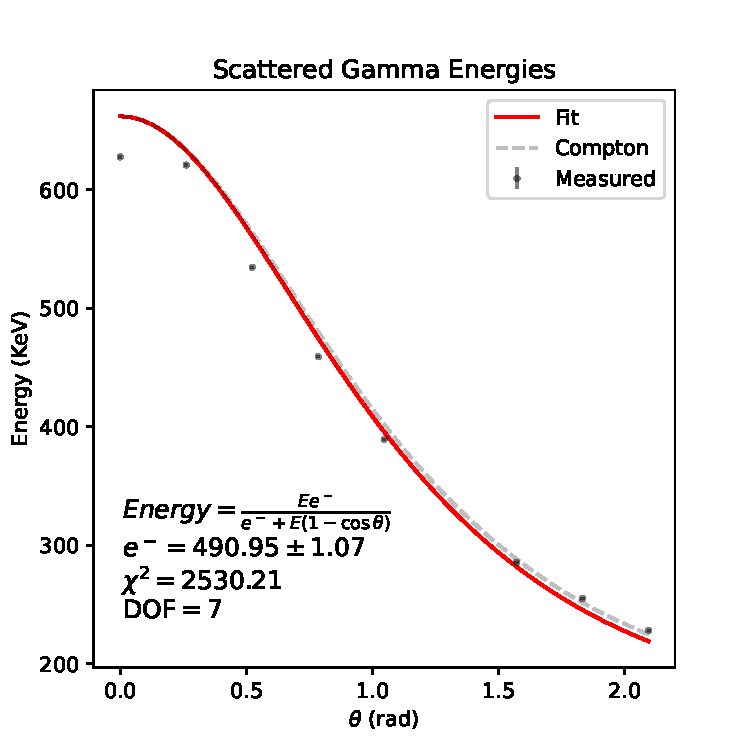
\includegraphics[width=0.75\textwidth]{experiment2/figures/compton_fit.pdf}
    \caption{Scattering data taken from setup with collimator. The calibration function is $\text{Energy} = 1.50 \cdot \text{Channel}-1.18$. }
    \label{fig:compton-fit}
\end{figure}

Now, the two curves looks fairly close. However, this seems only to be a relic of our model ansatz. It enforces a y-intercept of $662$ KeV, which drastically boosts its faithfulness to the Compton curve in the low angle regime. Furthermore, the low bias we achieve for large $\theta$ closer to $\pi$ helps the curve do well there as well. This is all at the cost of our error. The curve in effect ignores the data points around small $\theta$s, and accumulates a large error because of them. The reduced $\chi^2$ score is $361.46$, indicating a poor fit. 

It seems our issues all boil down to biases around small values of $\theta$. Though we were able to dispel the large overestimating bias via a intensity-reducing lead collimator, this revealed an underestimating bias which, though smalled in magnitude, continues to prove troubling. 

Our previous exploration of data-related issues, demonstrated by the inquiry into calibration error, proved unfruitful. We thus conjecture that these biases are inherent to our setup, as evidenced by our success culling PMT saturation. Going forward, we might seek to ensure the collimator is not interfering with photons to reduce their energy, which would explain the negative bias we observe. Or, we might continue to investigate the relationship between the gamma beam and the way the PMT measures it discretely. That is to say, we should look towards our success using the collimator, and use it as inspiration to continue our search. 

\end{document}

\begin{table}[!h]
\footnotesize
\centering
\begin{tabular}{| c | c c | c |}
    \hline
    $\theta$ (deg) & Centroid & Gain & \textbf{Channel} \\
    \hline
    0 & $833.09 \pm 0.09$ & 2 & $416.55 \pm 0.04$ \\
    15 & $823.98 \pm 0.22$ & 2 & $411.99 \pm 0.11$ \\
    30 & $709.66 \pm 0.30$ & 2 & $354.83 \pm 0.15$ \\
    45 & $609.79 \pm0.29$ & 2 & $304.89 \pm 0.14$ \\
    60 & $517.41 \pm 0.29$ & 2 & $258.70 \pm 0.14$ \\
    90 & $379.66 \pm 0.30$ & 2 & $189.83 \pm 0.15$ \\
    105 & $339.31 \pm 0.48$ & 2 & $169.66 \pm 0.24$ \\
    120 & $303.96 \pm 0.45$ & 2 & $151.98 \pm 0.23$ \\
    \hline 
\end{tabular}
\caption{Table of scattering measurements taken from setup with collimator. Centroid denotes the fitted peak mean $\mu$ and $\text{Channel}=\text{Centroid}/\text{Gain}$}
\label{table:scattering3}
\end{table}